\appendix

\chapter{Annexe de la partie 1. Rappels\,: ensembles de nombres.}\label{app_nbs}

	\section{Nombres entiers naturels}
		Les nombres naturels servent à compter des quantités dénombrables. Ils ont été l'objet de la première séance de \guil{maths-champignons}. Nous en donnons une définition concise ici, qui prend le risque d'être circulaire.
		\begin{defi}
			L'ensemble des nombres entiers naturels est l'ensemble des nombres que l'on peut obtenir, partant de zéro, par une succession arbitraire d'additions d'unité.

			Cet ensemble est noté symboliquement $\N$.
		\end{defi}
		\paragraph{Remarques.} 

		\begin{itemize}[label=\textbullet]
			\item Dans cette définition, on considère \guil{succession arbitraire} au sens large, en y incluant l'absence de succession. Ce qui fait que $O$ est également un entier naturel.
			\item Dans de nombreux livres de mathématiques, on peut souvent lire\,: $\N=\{0;1;2;\ldots\}$. En fait, presque tous les nombres entiers naturels sont dans les \guil{\ldots}\,!!! 
		\end{itemize}	


		Partant du repère cartésien à une dimension, on peut proposer cette définition alternative\,:
		\begin{defi}
			Considérons une droite graduée $(O;I)$ où par convention, $OI$ représente l'unité. L'ensemble des nombres entiers naturels est l'ensemble des abscisses des points obtenus par une succession quelconque de translations de bipoint $(O;I)$ --- c'est-à-dire la translation qui transforme $O$ en $I$.
		\end{defi}

		Nous donnons une illustration géométrique de cette définition ci-dessous.
		
		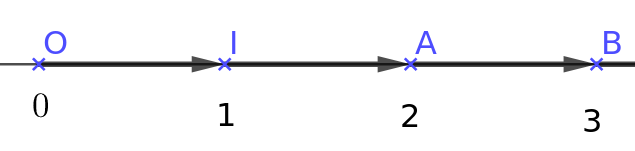
\includegraphics[width=0.5\textwidth]{image/calcul/ens_N.png} 

	\section{Nombres entiers relatifs}
		L'ensemble des nombres entiers relatifs introduit la notion de nombres négatifs. Pour les introduire, on peut considérer le problème suivant\,: trouver un nombre $a$ tel que $3+a=2$ (nous laissons le lecteur réfléchir à ce problème).

		\begin{defi}
			L'ensemble des nombres entiers relatifs est l'ensemble des nombres qui peuvent s'obtenir, partant de zéro, par successions arbitraires d'additions ou soustractions d'unité.

			De manière équivalente, étant donné une droite graduée $(O;I)$ avec $OI$ l'unité, c'est l'ensemble des abscisses des points qui peuvent être obtenus, partant de $O$, par une succession arbitraire de translations de bipoints $(0;I)$ ou $(I;O)$.

			Cet ensemble est noté $\Z$.
		\end{defi} 

		\paragraph{Remarque.} Dans les livres de mathématiques, on lit souvent \\ $\Z=\{\ldots;-3;-2;-1;0;1;2,3;\ldots\}$. Même remarque\,: presque tous les nombres sont cachés dans les \guil{\ldots}.

		\vspace{0.3cm}

		On donne une illustration de l'ensemble $\Z$ ci-dessous.

		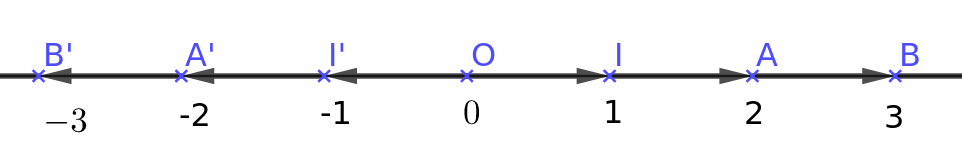
\includegraphics[width=0.8\textwidth]{image/calcul/ens_Z.png}


	\section{Nombres rationnels}
		Considérons deux nombres entiers $p$ et $q$ avec $q$ non nul. Nous allons proposer une construction géométrique qui permet de placer un point dont l'abscisse est le résultat de la division de $p$ par $q$.

		Placer deux points $O$, $I$ distincts sur le plan. Tracer une droite numérique orientée $(O;I)$. $OI$ sera l'unité. Placer un autre point $J$ hors de la droite $(OI)$ tel que $OJ=OI$. Tracer la droite numérique orientée $(O;J)$. Il n'est pas nécessaire que $(OI)\perp (OJ)$. Sur la droite numérique $(O;I)$, placer le point $P$ d'abscisse $x_P=p$. Sur la droite numérique $(O;J)$, placer le point $Q$ d'abscisse $x_Q=q$. Tracer la droite $(JP)$. Tracer la droite $(d)$ passant par $Q$ et parallèle à la droite $(JP)$. Placer $A=(d)\cap(OI)$. Alors l'abscisse de $A$ vaut $p/q$ (illustration figure \ref{fig_psq}).

		\begin{figure}
			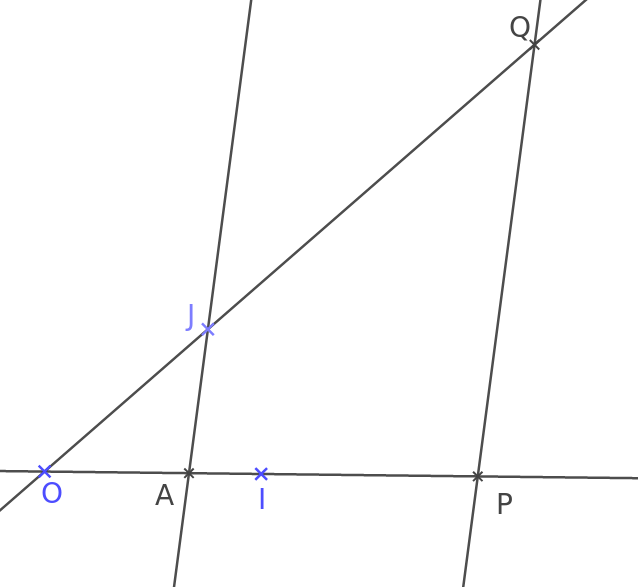
\includegraphics[width=0.6\textwidth]{image/calcul/constr_psq.png}
			\caption{Pour cette construction, on a pris $p=2$ et $q=3$. L'abscisse de $A$ vaut donc $2/3$.}
			\label{fig_psq}
		\end{figure}

		\begin{proof}
			On se contente de démontrer le résultat dans le cas où $p$ et $q$ sont strictement positifs. Nous laissons les autres cas aux lecteurs, les démonstrations étant analogues.

			Les cas $p=q=1$ étant triviaux, on suppose que $p$ ou $q$ est strictement supérieur à 1. Dans ce cas, les points $O$, $A$, $P$ sont alignés dans le même ordre que les points alignés $O$, $J$ $Q$ (sinon, les droites $(JA)$ et $(PQ)$ seraient sécantes). Comme les droites $(JA)$ et $(PQ)$ sont parallèles, on peut utiliser le théorème de Thalès\,:
			\begin{equation}
				\frac{OA}{OP}=\frac{OJ}{OQ}
			\end{equation}
			Donc
			\begin{equation}
				\frac{OA}{OJ}=\frac{OA}{OI}=\frac{OP}{OQ}=\frac{p}{q}
			\end{equation}
			(car $OI=OJ$). Et donc, l'abscisse du point $A$ est bien $p/q$.
		\end{proof}

		On peut en déduire la définition suivante\,:
		\begin{defi}
			L'ensemble des nombres rationnels est l'ensemble des abscisses des points qui peuvent s'obtenir par la construction précédente, avec $p\in\Z$, et $q\in\N\backslash\{0\}$ (tous les nombres entiers naturels sauf $0$).

			On note $\Q$ cet ensemble.

			De manière équivalente, on peut écrire\,:
			\begin{equation}
				\Q=\left\{\left.\frac{p}{q}\right|p\in\Z, q\in\N\backslash\{0\}\right\},
			\end{equation}
			soit l'ensemble des nombres qui peuvent s'écrire sous la forme d'un quotient de nombres entiers.

		\end{defi}

	\section{Nombres décimaux}
		Les nombres décimaux sont les nombres utilisés par les physiciens. De manière intuitive, ce sont les nombres qui peuvent s'écrire avec \guil{un nombre fini de chiffres après la virgule}. Cela signifie qu'on a une précision limitée. On peut écrire cela de manière plus formelle.

		\begin{defi}
			Soit $(O;I)$ une droite graduée avec $OI$ l'unité. L'ensemble des nombres décimaux est l'ensemble des abscisses des points qui peuvent correspondre à un ensemble arbitraire de subdivisions récursives des intervalles entres les nombres entiers relatifs. 

			On note $\D$ cet ensemble de nombres.

			Autrement dit, 
			\begin{equation}
				\D=\left\{\left.\frac{a}{10^n}\right| a\in\N, n\in\Z\right\}
			\end{equation}
		\end{defi}

		\paragraph{Remarque.} Certains nombres rationnels sont aussi des nombres décimaux. Par exemple, $1/5=0.2$. En revanche, certains nombres rationnels, si on voulait les écrire sous forme décimale, auraient un nombre infini de chiffres après la virgule. En effet, lorsqu'on pose et qu'on effectue la division de 1 par 3, on trouve que $1/3=0.333\ldots$ à l'infini.

		\begin{thm}
			Soit $r/q$ la fraction irréductible d'un nombre rationnel. Alors ce nombre est décimal si et seulement si $q$ peut s'écrire sous la forme $2^k5^\ell$ où $k$ et $\ell$ sont des nombres entiers naturels. En langage plus formel\,:
			\begin{equation}
				\frac{r}{q}\in\D \Leftrightarrow \exists k,\ell\in\N, q=2^k5^\ell.
			\end{equation}
		\end{thm}
		\begin{proof}
			On présente deux démonstrations. La première procède par double inclusion d'ensembles, la seconde utilise des théorèmes classiques d'arithmétique.
			
			\noindent\emph{Première démonstration\,: double inclusion.}

			Soit $\D_0$ l'ensemble des nombres qui peuvent s'écrire sous la forme $\frac{a}{2^k5^\ell}$, où $a\in\Z, k,\ell\in\N$. Nous allons montrer que $\D_0=\D$. Pour montrer que deux ensembles sont égaux, il faut montrer que l'un est inclus dans l'autre et que l'autre est inclus dans l'un. Formellement, il faut donc montrer que $\D_0=\D\Leftrightarrow (\D\subset\D_0\wedge\D_0\subset\D)$. Alors, on aura démontré que tout nombre dans $\D$ peut s'écrire comme le demande le théorème, et que tout  nombre écrit comme le demande le théorème est bien un nombre décimal.

			Démontrons que $\D_0\subset\D$. Soit un nombre $x$, arbitraire, appartenant à $\D_0$\,; nous allons démontrer qu'il appartient aussi à $\D$. Comme $x\in\D_0$, on peut écrire $x=\frac{a}{2^k5^\ell}$. Mais\,:
			\begin{equation}
				x=\frac{a}{2^k5^\ell}=\frac{a}{2^k5^\ell}\cdot\frac{2^{k\ell}5^{k\ell}}{2^{k\ell}5^{k\ell}}=\frac{a 2^{k\ell-k}5^{k\ell-\ell}}{2^{k\ell}5^{k\ell}}=\frac{a2^{k\ell-k}5^{k\ell-\ell}}{(2\times 5)^{k\ell}}=\frac{a2^{k\ell-k}5^{k\ell-\ell}}{10^{k\ell}},
			\end{equation}
			le numérateur étant un nombre entier et le dénominateur une puissance de dix, on a bien $x\in\D$. Donc $\D_0\subset\D$.

			Démontrons maintenant que $\D\subset\D_0$. Soit $y\in\D_0$\,; on peut écrire $y=\frac{b}{10^n}$ où $b\in\Z$ et $n\in\N$. Alors\,:
			\begin{equation}
				y=\frac{b}{10^n}=\frac{b}{(2\times 5)^n}=\frac{b}{2^n5^n}
			\end{equation}
			donc $b\in\D_0$. Donc $\D\subset\D_0$

			Conclusion\,: $\D=\D_0$.

			\noindent\emph{Deuxième démonstration\,: arithmétique.}
			
			$\Leftarrow$ On sait que $1/5=0.2$ et que $1/2=0.5$. $\D$ est stable par multiplication, donc pour tous $k,\ell\in\N$, $r/(2^k5^\ell)\in\D$.

			$\Rightarrow$ ($\star$) Pour démontrer l'implication directe, on va procéder par contraposition absurde\,: on va démontrer la contraposée (que si le dénominateur ne s'écrit pas comme un produit de 2 et de 5, alors la fraction n'est pas rationnelle) par l'absurde (on va supposer que le dénominateur du nombre ne s'écrit pas ainsi mais est quand même rationnel, et aboutir à une contradiction).

			Soit donc
			\begin{equation}
				q=\prod_i p_i^{k_i}
			\end{equation} 
			la décomposition en facteurs premiers du dénominateur de $r/q$. Supposons que les $p_i$ ne soient pas que des diviseurs de 10, soit $p$ l'un d'entre eux (non diviseur de 10). On récrit $q=p^kS$, avec 
			\begin{equation}
			 S=\prod_{p_i\ne p}p_i^{k_i}.\end{equation} 
			Supposons que $r$ soit un nombre décimal. Alors, on aurait
			\begin{equation}
				\frac{a}{10^n}=\frac{r}{p^kS}
			\end{equation}
			avec $a\in\Z$ et $n\in\N$, et donc $ap^kS=r10^n$ (axiome du produit en croix).
			La fraction étant réputée irréductible, $p$ et $r$ sont premiers entre eux, donc $p^k$ est un diviseur de $10^n$, or la décomposition (unique) en facteurs premiers de $10^n$ est $2^n5^n$, donc $p=2$ ou $p=5$. Mais on avait supposé que $p$ n'était pas un diviseur de 10. Contradiction. 
		\end{proof}

	\section{Nombres réels}
		Comme nous l'avons vu lors de \guil{maths-champignons}, il existe des nombres irrationnels, c'est-à-dire qu'on peut construire des longueurs qui ne peuvent pas s'exprimer sous la forme d'un rapport de nombres entiers. De manière synthétique (nous développerons ce point dans une session ultérieure de notre école de mathématiques), on peut dire que l'ensemble des nombres réels constitue \guil{toutes} les abscisses possibles sur la droite graduée.

	\section{Résultats sur les ensembles de nombres.}

		\begin{thm}
			$\N\subset\Z\subset\D\subset\Q\subset\R$. Cela signifie que l'ensemble $\N$ est contenu dans l'ensemble $\Z$, qui lui-même est contenu dans $\D$, lui-même contenu dans $\Q$, lui-même contenu dans $\R$.
		\end{thm}
		\begin{proof}
			Très élémentaire, donc laissée au lecteur.
		\end{proof}

		On trouve de nombreuses figures classiques sous forme de patatoïdes imbriquées pour illustrer cette inclusion. En voici une\,:




		Il existe d'autres ensembles de nombres encore plus gros. En effet, même si on peut démontrer que $\R$ n'a pas de trous, il lui manque quand même quelque chose. En effet, par exemple, l'équation $z^2=-1$ n'a pas de solution dans $\R$.

		\begin{proof}
			On raisonne par disjonction de cas. Un nombre réel $z$ est soit nul, soit strictement positif, soit strictement négatif. Il suffit donc de voir ce qui se passe pour chacun de ces trois cas.
			\begin{itemize}[label=\textbullet]
				\item Si $z=0$, alors $z^2=0$. Donc $z$ n'est pas solution.
				\item Si $z>0$, alors $z^2>0$. Donc $z$ n'est pas solution.
				\item Si $z<0$, alors $z^2>0$ également (car les deux signes moins multipliés donnent un signe plus). Donc $z$ n'est pas solution.
			\end{itemize}
			Ainsi, aucun des nombres réels ne peut vérifier l'égalité demandée. Il n'y a donc pas de solution.
		\end{proof}

		Eh bien, il existe un ensemble de nombres qui peut \guil{compléter} l'ensemble $\R$ pour que toutes les équations dites algébriques (comme celle que nous venons de voir) aient forcément une solution. On appelle cet ensemble l'ensemble des nombres \guil{complexes}, et on le note $\C$. Le nombre le plus important de cet ensemble est le nombre $\i$, qui vérifie justement $\i^2=-1$.

		Pour plus d'informations sur les nombres complexes, consulter par exemple la vidéo suivante\,:\url{https://www.youtube.com/watch?v=7BaaJ00nONE}. Toute la saga vaut largement le détour\,: \url{https://www.youtube.com/watch?v=cL7BpDrRc4s&list=PLw2BeOjATqrtiLPWvH_VeXmmBRmwcEwLz}.


\chapter{Annexes de : $\pi$ est un nombre}
\section{Flocon de Koch}\label{app_flocon}
Le flocon de Koch est un exemple de figure continue, qui occupe une aire finie, mais dont le périmètre est infini. Ce flocon s'obtient par itérations en partant d'un triangle équilatéral, et en ajoutant des triangles équilatéraux un tiers plus petit à chaque fois sur chaque côté.

Pour plus d'informations\,: \url{https://fr.wikipedia.org/wiki/Flocon_de_Koch}

\begin{figure}[h!]
	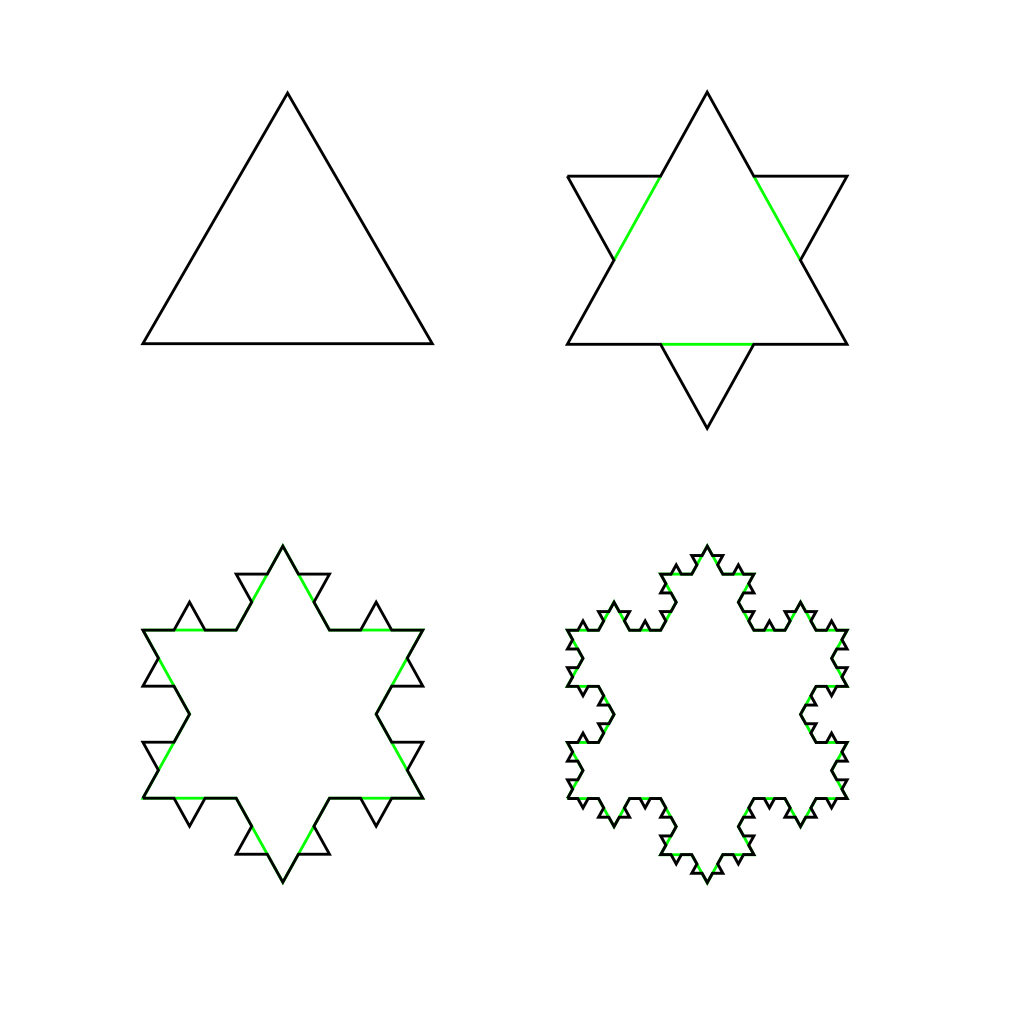
\includegraphics[width=0.6\textwidth]{image/pi_nombre/koch.png}
	\caption{Quatre premières itérations du flocon de Koch.}
\end{figure}

\section{Convergence des périmètres}\label{app_conv}

Dans cette section, $n$ désigne un entier naturel quelconque, et $(z_n)$ désigne une suite numérique de terme général $z_n$.


Il s'agit de démontrer que les suites $(P_n)$ et $(L_n)$ convergent vers la même limite. 


Par construction et par inégalité triangulaire, il est évident que $L_{n+1}>L_n$ et que $P_{n+1}<P_n$. Ainsi, $(L_n)$ est croissante et $(P_n)$ est décroissante. $(P_n)$ est minorée (car positive) donc converge. 
$L_n$ et $P_n$ correspondent aux périmètres de polygones réguliers à $6\times 2^n$ côtés. Le polygone correspondant à $P_n$ est obtenu par une homothétie de rapport supérieur à 1 appliquée à celui correspondant à $L_n$. Donc $L_n<P_n<P_0$ donc $(L_n)$ est majorée. Donc $(L_n)$ converge.

À présent que nous savons que ces deux suites convergent vers des valeurs non nulles, il s'agit de démontrer que c'est la même valeur.

Commençons par remarquer que d'après \eqref{eq_cnpu} et \eqref{eq_dnpu}, et en n'oubliant pas que $L_n=6\times2^n c_n$ et $P_n=6\times 2^n d_n$, on obtient\,:
\begin{align}
	P_{n+1}&=\sqrt{2}\sqrt{\sqrt{\frac{P_n^2}{3^22^{2n+4}}+1}-1},\\
	L_{n+1}&=\sqrt{2}\sqrt{1-\sqrt{1-\frac{L_n^2}{3^22^{2n+4}}}}.
\end{align}
De là, nous obtenons
\begin{equation}
	\frac{P_{n+1}^2-L_{n+1}^2}{2}=\sqrt{1+x_n}+\sqrt{1-y_n}-2
\end{equation}
en ayant posé 
\begin{equation}
	x_n=\frac{P_n^2}{3^22^{2n+4}};\quad y_n=\frac{L_n^2}{3^22^{2n+4}}.
\end{equation}
Comme les suites $(L_n)$ et $(P_n)$ convergent, les suites $(x_n)$ et $(y_n)$ convergent vers 0. Mais
\begin{equation}
	\sqrt{1+x_n}+\sqrt{1-y_n}-2\convn{0}.
\end{equation}
Donc $\frac{P_{n+1}^2-L_{n+1}^2}{2}\convn{0}$ et donc $(P_n)$ et $(L_n)$, suites positives qui convergent, ont la même limite.
On peut donc véritablement poser
\begin{equation}
	\boxed{\pi=\lim\limits_{n\to\infty}P_n=\lim\limits_{n\to\infty}L_n}.
\end{equation}

